\chapter{Interfaz gráfica}
\label{ch:ui}

\section{Análisis}
\label{sec:ui_analisis}

En esta sección se comenzará a trabajar en la aplicación, realizando en primer lugar un breve análisis para concretar sus requisitos.

En el caso de la interfaz gráfica, el ámbito de uso difiere un poco del concretado para el firmware en la sección \ref{sec:fw_analisis}. Esta se pretende usar desde Valeo para incluir en el dispositivo las ranuras que cada fabricante necesite antes de proporcionarles el PWM Box. Por lo tanto, se deduce que su uso va a ser en un entorno algo más administrativo que en el caso anterior.

Si bien se anticipa, por lo tanto, que el usuario tenga un mayor nivel de entendimiento a la hora de manejar sistemas informáticos, sigue sin esperarse ningún tipo de conocimiento técnico. Solamente se asumirá algo de destreza en el uso de programas de ofimática y similares.

Teniendo esto en cuenta, se determinarán los requisitos de la aplicación.

\subsubsection{Comunicación con el dispositivo}
\label{subsub:ui_requisitos}

\begin{table}[h!]
    \centering
    \caption{RF-1. Conectar con el dispositivo.}
    \begin{tabular}{|m{2.5cm}|m{9.27cm}|}
        \hline
        \textbf{ID} & RF-1 \\
        \hline
        \textbf{Nombre} & Conectar con el dispositivo \\
        \hline
        \textbf{Descripción} & El sistema debe ser capaz de encontrar el puerto del dispositivo en el equipo y conectarse a él de forma automática, tanto desde Windows como desde Linux. \\
        \hline
        \textbf{Prioridad} & Alta \\
        \hline
    \end{tabular}
\end{table}

\begin{table}[h!]
    \centering
    \caption{RF-2. Obtener la información básica del dispositivo.}
    \begin{tabular}{|m{2.5cm}|m{9.27cm}|}
        \hline
        \textbf{ID} & RF-2 \\
        \hline
        \textbf{Nombre} & Obtener la información básica del dispositivo \\
        \hline
        \textbf{Descripción} & El sistema debe poder obtener la información básica del dispositivo. Esto incluye su número de serie, su versión de \textit{hardware} y su versión de \textit{software}. \\
        \hline
        \textbf{Prioridad} & Alta \\
        \hline
    \end{tabular}
\end{table}

\begin{table}[h!]
    \centering
    \caption{RF-3. Obtener la configuración general del dispositivo.}
    \begin{tabular}{|m{2.5cm}|m{9.27cm}|}
        \hline
        \textbf{ID} & RF-3 \\
        \hline
        \textbf{Nombre} & Obtener la configuración general del dispositivo \\
        \hline
        \textbf{Descripción} & El sistema debe tener la capacidad de obtener la configuración general del dispositivo, que consiste de su contraseña y la ranura por defecto establecida. \\
        \hline
        \textbf{Prioridad} & Alta \\
        \hline
    \end{tabular}
\end{table}

\begin{table}[h!]
    \centering
    \caption{RF-4. Obtener las ranuras guardadas en el dispositivo.}
    \begin{tabular}{|m{2.5cm}|m{9.27cm}|}
        \hline
        \textbf{ID} & RF-4 \\
        \hline
        \textbf{Nombre} & Obtener las ranuras guardadas en el dispositivo \\
        \hline
        \textbf{Descripción} & El sistema debe comunicarse con el dispositivo para obtener las ranuras que estén guardadas en la memoria del mismo, incluyendo la información relativa a las señales PWM que las componen. \\
        \hline
        \textbf{Prioridad} & Alta \\
        \hline
    \end{tabular}
\end{table}

\begin{table}[h!]
    \centering
    \caption{RF-5. Enviar configuración general al dispositivo.}
    \begin{tabular}{|m{2.5cm}|m{9.27cm}|}
        \hline
        \textbf{ID} & RF-5 \\
        \hline
        \textbf{Nombre} & Enviar configuración general al dispositivo \\
        \hline
        \textbf{Descripción} & El sistema debe ser capaz de enviar de vuelta al dispositivo su configuración general. \\
        \hline
        \textbf{Prioridad} & Alta \\
        \hline
    \end{tabular}
\end{table}

\begin{table}[h!]
    \centering
    \caption{RF-6. Enviar ranuras al dispositivo.}
    \begin{tabular}{|m{2.5cm}|m{9.27cm}|}
        \hline
        \textbf{ID} & RF-6 \\
        \hline
        \textbf{Nombre} & Enviar ranuras al dispositivo \\
        \hline
        \textbf{Descripción} & El sistema debe poder enviar ranuras configuradas al dispositivo. \\
        \hline
        \textbf{Prioridad} & Alta \\
        \hline
    \end{tabular}
\end{table}

\subsubsection{Gestión del dispositivo}

\begin{table}[h!]
    \centering
    \caption{RF-7. Mostrar la información básica del dispositivo.}
    \begin{tabular}{|m{2.5cm}|m{9.27cm}|}
        \hline
        \textbf{ID} & RF-7 \\
        \hline
        \textbf{Nombre} & Mostrar la información básica del dispositivo \\
        \hline
        \textbf{Descripción} & El sistema debe permitir al usuario consultar la información básica del dispositivo. \\
        \hline
        \textbf{Prioridad} & Alta \\
        \hline
    \end{tabular}
\end{table}

\begin{table}[h!]
    \centering
    \caption{RF-8. Mostrar la configuración general del dispositivo.}
    \begin{tabular}{|m{2.5cm}|m{9.27cm}|}
        \hline
        \textbf{ID} & RF-8 \\
        \hline
        \textbf{Nombre} & Mostrar la configuración general del dispositivo \\
        \hline
        \textbf{Descripción} & El sistema debe permitir al usuario visualizar la configuración general del dispositivo. \\
        \hline
        \textbf{Prioridad} & Alta \\
        \hline
    \end{tabular}
\end{table}

\begin{table}[h!]
    \centering
    \caption{RF-9. Mostrar los parámetros de las señales generadas.}
    \begin{tabular}{|m{2.5cm}|m{9.27cm}|}
        \hline
        \textbf{ID} & RF-9 \\
        \hline
        \textbf{Nombre} & Mostrar los parámetros de las señales generadas \\
        \hline
        \textbf{Descripción} & El sistema debe mostrar al usuario los parámetros de las distintas señales PWM configuradas. \\
        \hline
        \textbf{Prioridad} & Alta \\
        \hline
    \end{tabular}
\end{table}

\subsubsection{Gestión de ranuras}

\begin{table}[h!]
    \centering
    \caption{RF-10. Crear ranuras nuevas.}
    \begin{tabular}{|m{2.5cm}|m{9.27cm}|}
        \hline
        \textbf{ID} & RF-10 \\
        \hline
        \textbf{Nombre} & Crear ranuras nuevas \\
        \hline
        \textbf{Descripción} & Crear ranuras nuevas. \\
        \hline
        \textbf{Prioridad} & Alta \\
        \hline
    \end{tabular}
\end{table}

\begin{table}[h!]
    \centering
    \caption{RF-11. Exportar ranuras al equipo.}
    \begin{tabular}{|m{2.5cm}|m{9.27cm}|}
        \hline
        \textbf{ID} & RF-11 \\
        \hline
        \textbf{Nombre} & Exportar ranuras al equipo \\
        \hline
        \textbf{Descripción} & El sistema debe permitir exportar las ranuras cargadas a la memoria del equipo en un formato adecuado. \\
        \hline
        \textbf{Prioridad} & Alta \\
        \hline
    \end{tabular}
\end{table}
\label{tab:rf11}

\begin{table}[h!]
    \centering
    \caption{RF-12. Importar ranuras del equipo.}
    \begin{tabular}{|m{2.5cm}|m{9.27cm}|}
        \hline
        \textbf{ID} & RF-12 \\
        \hline
        \textbf{Nombre} & Importar ranuras del equipo \\
        \hline
        \textbf{Descripción} & El sistema debe permitir al usuario importar las ranuras almacenadas con un determinado formato en la memoria del equipo. \\
        \hline
        \textbf{Prioridad} & Alta \\
        \hline
    \end{tabular}
\end{table}
\label{tab:rf12}

\begin{table}[h!]
    \centering
    \caption{RF-13. Visualizar la configuración de las ranuras.}
    \begin{tabular}{|m{2.5cm}|m{9.27cm}|}
        \hline
        \textbf{ID} & RF-13 \\
        \hline
        \textbf{Nombre} & Visualizar la configuración de las ranuras \\
        \hline
        \textbf{Descripción} & El sistema permitir al usuario consultar los parámetros de las señales PWM que componen las ranuras cargadas. \\
        \hline
        \textbf{Prioridad} & Alta \\
        \hline
    \end{tabular}
\end{table}

\begin{table}[h!]
    \centering
    \caption{RF-14. Modificar los parámetros de las ranuras cargadas.}
    \begin{tabular}{|m{2.5cm}|m{9.27cm}|}
        \hline
        \textbf{ID} & RF-14 \\
        \hline
        \textbf{Nombre} & Modificar los parámetros de las ranuras cargadas \\
        \hline
        \textbf{Descripción} & El sistema debe permitir la creación de ranuras nuevas desde la propia aplicación. \\
        \hline
        \textbf{Prioridad} & Alta \\
        \hline
    \end{tabular}
\end{table}

\FloatBarrier

\subsubsection{Requisitos no funcionales}

\begin{table}[h!]
    \centering
    \caption{RNF-1. Manejabilidad.}
    \begin{tabular}{|m{2.5cm}|m{9.27cm}|}
        \hline
        \textbf{ID} & RNF-1 \\
        \hline
        \textbf{Nombre} & Manejabilidad \\
        \hline
        \textbf{Descripción} & El sistema ha de ser sencillo e intuitivo para los usuarios. \\
        \hline
        \textbf{Prioridad} & Alta \\
        \hline
    \end{tabular}
\end{table}

\begin{table}[h!]
    \centering
    \caption{RNF-2. Rendimiento.}
    \begin{tabular}{|m{2.5cm}|m{9.27cm}|}
        \hline
        \textbf{ID} & RNF-2 \\
        \hline
        \textbf{Nombre} & Rendimiento \\
        \hline
        \textbf{Descripción} & El sistema debe ser fluido y responder a las acciones del usuario sin demoras excesivas. \\
        \hline
        \textbf{Prioridad} & Alta \\
        \hline
    \end{tabular}
\end{table}

\begin{table}[h!]
    \centering
    \caption{RNF-3. Aspecto atractivo.}
    \begin{tabular}{|m{2.5cm}|m{9.27cm}|}
        \hline
        \textbf{ID} & RNF-3 \\
        \hline
        \textbf{Nombre} & Aspecto atractivo \\
        \hline
        \textbf{Descripción} & El sistema debe ser atractivo visualmente. \\
        \hline
        \textbf{Prioridad} & Media \\
        \hline
    \end{tabular}
\end{table}

\section{Diseño}
\label{sec:ui_diseño}

La fase de diseño de la interfaz comienza con un prototipado visual de la aplicación. Teniendo en cuenta el análisis realizado, se plantea mantener un aspecto simple, estando la información acerca de las distintas señales en una misma ventana. De esta forma, todos los aspectos de interés se encontrarán a simple vista, evitando que el usuario pierda tiempo innecesariamente para encontrar la información que busca. Esto se considera especialmente apropiado para el entorno al que se destina el producto.

Las distintas operaciones adicionales, como enviar perfiles al dispositivo o exportar archivos, sí se realizarán en ventanas separadas. Aún así, la complejidad de las mismas se mantendrá al mínimo, haciéndolas lo más intuitivas posible.

Con todo ello, el primer prototipo al que se llega puede verse en la figura \ref{fig:ui_diseño1}. Sobre este se realizan numerosas iteraciones, centrándonos primero en incluir todas las funcionalidades necesarias, y posteriormente, en mejorar el aspecto, manejabilidad y accesibilidad de la interfaz en general. En las figuras \ref{fig:ui_diseño2} y \ref{fig:ui_diseño3} se pueden ver dos ejemplos de este proceso, hasta llegar a la versión final, mostrada en las figuras \ref{fig:ui_diseño_final1} y \ref{fig:ui_diseño_final2}.

\begin{figure}[h!]
    \centering
    \includegraphics[width=0.95\textwidth]{ui_diseño1.png}
    \caption{Primera iteración del diseño de la interfaz.}
    \label{fig:ui_diseño1}
\end{figure}


\begin{figure}[h!]
    \centering
    \includegraphics[width=0.95\textwidth]{ui_diseño2.png}
    \caption{Otra iteración del diseño de la interfaz.}
    \label{fig:ui_diseño2}
\end{figure}

\begin{figure}[h!]
    \centering
    \includegraphics[width=0.95\textwidth]{ui_diseño3.png}
    \caption{Otra iteración del diseño de la interfaz.}
    \label{fig:ui_diseño3}
\end{figure}


\begin{figure}[h!]
    \centering
    \begin{subfigure}{0.95\textwidth}
        \includegraphics[width=0.95\textwidth]{ui_diseño4.png}
    \end{subfigure}
    \vfill
    \begin{subfigure}{0.95\textwidth}
        \includegraphics[width=0.95\textwidth]{ui_diseño5.png}
    \end{subfigure}
    \caption{Diseño final de la interfaz.}
\end{figure}
\label{fig:ui_diseño_final1}

\begin{figure}[h!]
    \centering
    \includegraphics[width=0.95\textwidth]{ui_diseño6.png}
    \caption{A la izquierda, ventana para exportar ranuras. A la derecha, ventana para enviar ranuras al dispositivo}
    \label{fig:ui_diseño_final2}
\end{figure}

\FloatBarrier

En cuanto al diseño del \textit{software} del sistema, la idea principal ha sido mantener la estructura general de los conceptos definidos para el dispositivo, con el objetivo de asegurar la compatibilidad de ambos desarrollos sin añadir complejidad innecesaria a la comunicación entre ambos. Los distintos módulos definidos se describen a continuación.

\subsection{PWM Types}

El primer aspecto a definir es la forma en la que se van a representar los PWM en esta parte del proyecto. Para ello, se crea el módulo PWM Types, cuyos objetos servirán como almacén de datos para las distintas señales PWM y perfiles cargados en la aplicación.

Un objeto de la clase PWM estará compuesto de la misma forma en la que se guardan las señales en la memoria del dispositivo (nombre, modo, frecuencia, ciclo, fase), pues estos son los parámetros externos que el usuario ha de ser capaz de modificar. De forma análoga, un objeto de la clase Slot contendrá su nombre y ocho objetos de la clase PWM.

\subsection{JSON Manager}

Para satisfacer los requisitos \hyperref[tab:rf11]{RF-11} y \hyperref[tab:rf12]{RF-12}, se plantea el uso de archivos JSON. Estos resultan una forma sencilla de almacenar datos estructurados en un formato legible, la cual se adecúa a la jerarquía establecida entre un perfil y sus señales.

\subsection{PWM Box}

Adicionalmente, se define el módulo PWM Box. Este servirá de unión entre las funcionalidades de la interfaz y las del dispositivo, realizando las labores de comunicación por el puerto serie.

De igual forma que el módulo PWM Types, su contenido será análogo al del dispositivo, conteniendo, de los datos que este almacena en memoria, aquellos a los que el usuario deba tener acceso.

\subsection{Main}

Por último, el módulo principal es el que controlará todas las características de la interfaz. Estará dividido en distintas clases, cada una de las cuales contendrá la funcionalidad de una ventana distinta. Se distinguen las siguientes:

\begin{itemize}
    \item\textbf{Ventana principal:} En ella se mostrará toda la información referente a las distintas señales PWM. Se permitirá al usuario escoger qué perfil está visualizando, así como realizar las distintas operaciones definidas en los \hyperref[subsub:ui_requisitos]{requisitos}.
    \item\textbf{Ventana de envío:} Permitirá al usuario elegir cuáles de los perfiles cargados en la aplicación serán enviados al dispositivo. Será una prioridad representar esta acción de la forma más intuitiva posible.
    \item\textbf{Ventana de exportación:} Servirá para seleccionar qué perfiles se van a exportar.
    \item\textbf{Ventana de contraseña:} Mostrará la contraseña del dispositivo, y permitirá cambiarla por una nueva. También se usará cuando se abra la aplicación sin haber establecido una contraseña anteriormente, para obligar al usuario a hacerlo.
\end{itemize}

También se plantea el uso de alguna ventana adicional para usar como pantalla de carga si resulta oportuno, en caso de detectar algún proceso que tarde en ejecutarse.

Otro aspecto a tener en cuenta antes de comenzar la implementación, es el flujo de ejecución general de la aplicación, especialmente en lo que a envío de datos al dispositivo se refiere. En un primer momento se distinguen dos opciones.

\subsubsection{Opción 1: Envío de datos continuo}

Se considera una forma más ``moderna'' de conceptualizar la aplicación. En ella, cualquier cambio realizado sobre los parámetros de las señales sería enviado automáticamente al dispositivo. De igual forma, las ranuras creadas se añadirían también de forma automática a este. Esto permitiría sustituir completamente los controles físicos del PWM Box.

Esta sería la opción adecuada para una aplicación más orientada al ocio, que se pretenda distribuir para el uso cotidiano de todo tipo de usuarios. En este caso la comodidad que este enfoque ofrece sería ventajosa.

\subsubsection{Opción 2: Envío de datos controlado}

En este modelo de funcionamiento, se prioriza el control del usuario sobre el dispositivo. Los cambios que se realicen en la aplicación tendrán que ser manualmente aplicados, asegurando que la forma en la que funcione el dispositivo en todo momento sea intencionada.

Este es el enfoque que se ha elegido finalmente para la interfaz, ya que se considera más apropiado para el contexto y la forma en el que se usará. De esta manera, la aplicación servirá más como un almacén de perfiles, que podrán ser cargados en un PWM Box cuando se necesiten. Esta opción se alinea más con las necesidades expresadas por Valeo.

\subsection{General}

Habiendo planteado los distintos módulos, las interacciones entre ellos pueden modelarse a través de los diagramas de secuencia que se muestran a continuación.

\begin{figure}[h!]
    \centering
    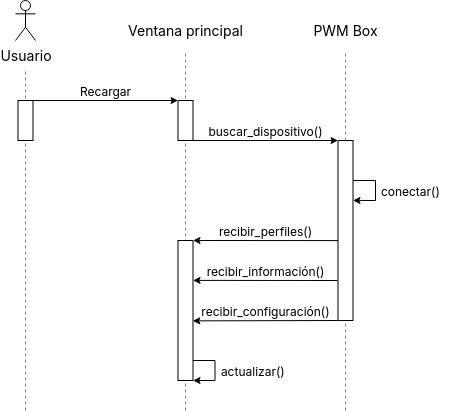
\includegraphics[width=\textwidth]{ui_recargar.png}
    \caption{Flujo de ejecución al recargar la conexión con el dispositivo.}
    \label{fig:ui_recargar}
\end{figure}

\begin{figure}[h!]
    \centering
    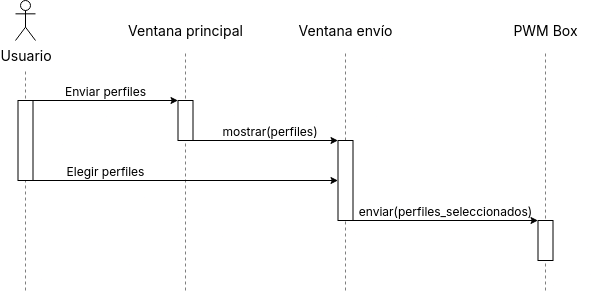
\includegraphics[width=\textwidth]{ui_enviar1.png}
    \caption{Flujo de ejecución al enviar perfiles al dispositivo.}
    \label{fig:ui_enviar1}
\end{figure}

\begin{figure}[h!]
    \centering
    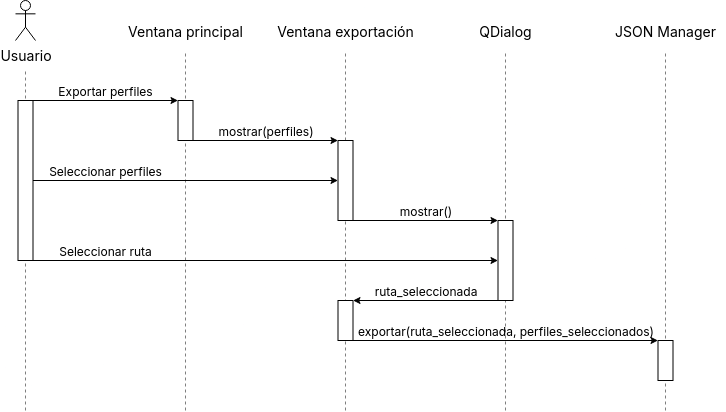
\includegraphics[width=\textwidth]{ui_exportar.png}
    \caption{Flujo de ejecución al exportar perfiles al equipo.}
    \label{fig:ui_exportar}
\end{figure}

\begin{figure}[h!]
    \centering
    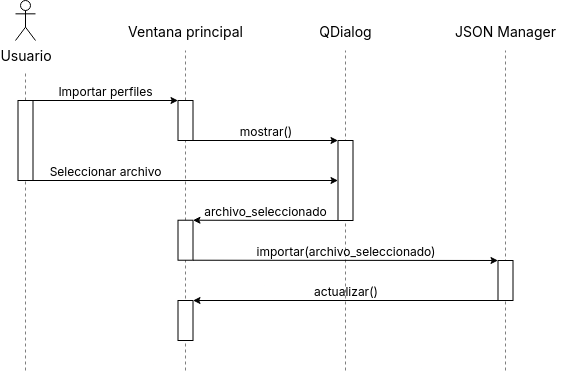
\includegraphics[width=\textwidth]{ui_importar.png}
    \caption{Flujo de ejecución al importar perfiles desde el equipo.}
    \label{fig:ui_importar}
\end{figure}

\begin{figure}[h!]
    \centering
    \includegraphics[width=\textwidth]{ui_contraseña.png}
    \caption{Flujo de ejecución al mostrar y modificar la contraseña.}
    \label{fig:ui_contraseña}
\end{figure}

\begin{figure}[h!]
    \centering
    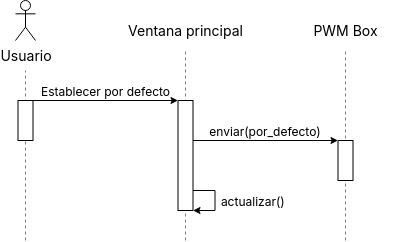
\includegraphics[width=\textwidth]{ui_por_defecto.png}
    \caption{Flujo de ejecución al establecer el perfil por defecto.}
    \label{fig:ui_por_defecto}
\end{figure}

\section{Desarrollo}

Para el desarrollo de la aplicación ha sido necesario el uso de la librería \textit{pyserial} \cite{pyserial-lib}. Las funcionalidades que proporciona han permitido gestionar todos los aspectos de la comunicación por el puerto serie.

También se ha hecho uso de la librería estándar \textit{json} \cite{json-lib} para la codificación y decodificación de los archivos en este formato.

Por último, para la apariencia general de la aplicación, se ha usado el tema \textit{catppuccin latte} de la librería \textit{qt-themes} \cite{qtthemes-lib}.

Durante el proceso de implementación se ha enfrentado una situación que no se había tenido en cuenta en la etapa de diseño: la forma de gestionar las distintas fuentes de las que puede provenir un perfil. Como se determinó en la definición de los \hyperref[subsub:ui_requisitos]{requisitos}, un perfil puede cargarse en la aplicación desde el dispositivo, desde un archivo importado, o puede ser directamente creado a través de la interfaz. Es conveniente manejar estas tres fuentes por separado, ya que cada una tiene ciertas peculiaridades. Por ejemplo, no tendría sentido permitir al usuario quitar de la aplicación un perfil que se encuentre cargado en el dispositivo, mientras que si lo tendría en el caso de tratarse de una ranura creada desde la interfaz.

Otro problema al que se ha hecho frente constituye una de las desventajas de la comunicación por el puerto serie: su velocidad. Se ha comprobado que al transmitir un número mayor de perfiles el proceso se alarga, llegando a bloquear momentáneamente el hilo de ejecución de la interfaz. Esto se debe a que el dispositivo necesita esperas entre cada envío de datos para recibirlos y procesarlos. Para intentar suavizarlo, se ha ajustado la recepción de datos del dispositivo, dejando el procesamiento más costoso para el final, una vez haya terminado la transmisión. Sin embargo, debido a la naturaleza de la adversidad, no se ha podido solucionar completamente.

Además, para evitar el bloqueo de la interfaz, se ha implementado la ejecución paralela de un hilo encargado de la comunicación por el puerto serie. Esto ha permitido también mostrar una ventana adicional, indicando al usuario que la transmisión de datos se encuentra en proceso.

\section{Pruebas}

En un primer lugar, se han ido llevando a cabo pruebas unitarias a lo largo del desarrollo, poniendo especial atención en los aspectos más transparentes al usuario (por ejemplo, el intercambio de datos con el dispositivo). Su objetivo ha sido evaluar el funcionamiento de los aspectos más esenciales, cuyos errores pueden resultar más difíciles de detectar en fases futuras del desarrollo.

Adicionalmente, tras completar cada funcionalidad general (envío de perfiles, exportación de archivos, etc.), se han realizado pruebas de integración para comprobar la validez del flujo de las operaciones, tal y como se han definido en los \hyperref[fig:ui_recargar]{diagramas de secuencia}.

Por último, cuando el desarrollo se ha completado, se han realizado pruebas de aceptación para asegurar el funcionamiento en conjunto de la aplicación, corrigiendo los pequeños errores encontrados.
